!en \section{Let there be light!}
!de \section{Es werde Licht!}

!en X

!de Das erste Beispiel in diesem Kapitel ist das kleinste Programm, das wir uns vorstellen können, das tatsächlich auch etwas sichtbares tut. Es wird die LED am Arduino Anschluss 13 einschalten.



!en X

!de In Assembler Programmieren heisst, die Macht zu haben! Doch wie wir wissen, erfordert Macht Wissen und Verantwortungsbewusstsein. Jemand der Micro Controller in Assembler programmiert, hat die absolute Macht über den Micro Controller, ob er es will oder nicht! Demzufolge ist ein Mindestmass an Fachwissen erforderlich um verantwortungsbewusst zu handeln. Da es unmöglich ist, von Anfang an gleich alles zu wissen, tasten wir uns vorsichtig vorwärts. Es gibt aber keinen Grund nicht beliebig im Buch vorwärts und Rückwärts zu blättern. Wir versuchen, die einzelnen Rezepte so unabhängig wie möglich und dennoch aufeinander aufbauend zu gestalten.



!en X

!de Als erstes müssen wir wissen, was der \textit{Digital Pin 13} am Arduino in Wirklichkeit ist. Infolge des Arduinodesigns ist Anschluss 13 am Arduino nicht Bein 13 am \at{}. Das tatsächliche Bein am \at{} zu kennen ist erforderlich um mit dem blanken Chip zu arbeiten. Darüber hinaus ist es erforderlich zu wissen, wie dieser Anschluss im Micro Controller adressiert werden muss. Um das alles heraus zu finden gibt es ein sehr schönes Schaubild: \url{http://www.arduino.cc/hu/Hacking/PinMapping}


\begin{figure}[htbp]
  \centering
  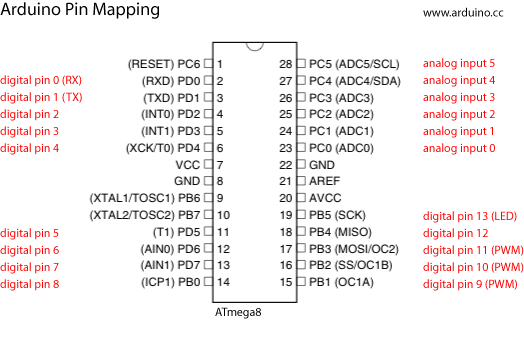
\includegraphics[width=120mm]{Media/www-arduino-cc_Arduino-To-Atmega8-Pins.png}
!en   \caption{Arduino to \at  pins}
!de   \caption{Arduino zu \at  Anschlusszuordnung}
  \label{arduino-to-atmega-pins}
\end{figure}



!en X

!de Nachdem wir zunächst vermutlich genug wissen um verantwortungsvoll zu handeln, programmieren wir unser 8 Byte grosses Programm, dass die LED am 'Arduino Digital Pin 13' erleuchtet.



\begin{lstlisting}
; LED/S000_let-there-be-light.asm

.DEVICE atmega8

.org 0x0000
            rjmp    start 

start:
            sbi     DDRB,         5
            sbi     PORTB,        5
            
main:
            rjmp    main
\end{lstlisting}


!en X

!de So einfach dieses Programm sein mag, es gibt doch ein paar Kleinigkeiten zu beleuchten.



!en X

!de Zunächst müssen wir angeben, welchen konkreten Micro Controller wir verwenden. Das ist erforderlich weil die verschiedenen Modelle verschiedene Adressen für ihre adressierbaren Elemente aufweisen. Dem Assembler wird auf diese Weise mitgeteilt, welche Werte er für welche Elemente verwenden muss. In unserem Beispiel für DDRB und PORTB. DDRB und PORTB sind Platzhalter oder auch 'logische Namen' für Zahlen. Welche Zahlen verwendet werden, entscheidet die Angabe des Micro Controllers hinter \texttt{.DEVICE}. Das geschieht durch:

\begin{lstlisting}
.DEVICE atmega8
\end{lstlisting}



!en X

!de Als nächstes müssen wir den Anfang der Welt benennen. Der Witz hierbei ist, dass wir die volle Wahrheit nie wirklich erfahren! Wir verwenden Symbole um mit dieser Anforderung umzugehen. Wie bereits beschrieben, haben verschiedene Micro Controller verschiedene innere Werte. Aber nicht nur das. Wo exakt sich unser Programm am Ende tatsächlich befinden wird, ist eine kaum beantwortbare Frage. Später werden wir nochmals darauf zurück kommen.


!en X:

!de Da wir also zur Verwendung von Symbolen gezwungen sind, werden wir dementsprechend handeln. Wir werden mit einem Symbol den Startpunkt unseres Programms markieren. Dieses Symbol werden wir 'start' nennen. Was immer auch unser Programm starten wird, es muss diesen Startpunkt kennen:

\begin{lstlisting}
.org 0x0000
            rjmp     start 
\end{lstlisting}



!en X

!de Mit '\texttt{.org}' (Bitte den Punkt am Anfang nicht vergessen!) eröffnen wir eine Liste von Befehlen, die an der bezeichnete Position (hier 0x0000) beginnt. Diese Liste, die auch Tabelle genannt wird, enthält Aktionen, die für beim Eintreten bestimmter Situationen ausgeführt werden sollen. Typischer Weise handelt es sich um Sprungbefehle. Die Situation, bzw, das Ereignis, dass in dieser Tabelle für unser Programm behandelt werden muss, ist, eben dieses Programm zu starten. Glücklicher Weise findet sich der Eintrag für die Aktion '\textit{Programm starten}'an der ersten Stelle diese Tabelle.


 
!en X

!de Dieses Vorgehen scheint auf den ersten Blich sonderbar. Wieso sollte man als erste Anweisung eines Programms zum Anfang des Programms springen müssen? Wieso nicht gleich das Programm starten? Sobald wir mit der Behandlung von Interrupts beginnen, wird das schnell verständlich werden.



!en X:

!de Für die Neugierigen: Die Adressierung innerhalb dieser Tabelle, ist immer relativ zum Anfang der Tabelle. Die Tabelle befindet sich in Wirklichkeit eher nicht an der Position \texttt{0x0000}, aber darauf müssen wir keine Rücksicht nehmen. Genau genommen betreten wir hier bereits eine Art Traumwelt: Wir wissen nicht wirklich, was passiert. Aber in manchen Fällen, wie hier, müssen wir das auch nicht wissen. Wir müssen uns lediglich bewusst sein, dass wir eben nicht wissen, wo im Speicher unsere Programme zu liegen kommen. Das wird wichtig, wenn Speicherzellen angesprochen werden müssen. So können wir die Adresse, an der unser Programm tatsächlich beginnt nicht kennen. Wir müssen des dem Assembler symbolisch erklären. Und zwar so:

\begin{lstlisting}
start:
\end{lstlisting}



!en X

!de '\texttt{start:}' ist eine Marke, ein 'Label'. In unserem Fall ist es eine Sprungmarke. Sie repräsentiert die Adresse der ersten Speicherstelle nach ihrem Erscheinen. In unserem Fall die Adresse des ersten Befehls unseres Programms. Der Assembler wird diese Adresse relativ adressieren, während sie beim Hochladen des Programms auf den Micro Controller in eine absolute Adresse umgewandelt wird.



!en X

!de Die nächste Sprungarke befindet sich bereits hinter dem eigentlichen Ende unseres Programms. Sie ist der Beginn einer unbedingten unendlichen Schleife. Diese Schleife ist erforderlich, weil der Prozessor (CPU) unseres Micro Controllers (MC) arbeitet, solange er Strom hat. Diese Aussage stimmt nicht, in Wirklichkeit kann man nicht nur die CPU anhalten. Das Anhalten der CPU ist aber bereits ein recht komplizierter Vorgang. Wichtig, aber kompliziert. Darum wollen wir hier so tun als wäre es nicht möglich. Da wir die CPU also (momentan) nicht stoppen können, müssen wir ihr etwas zu tun geben was das Ergebnis unseres Programms nicht beeinträchtigt.



!en 

!de Zwischen '\texttt{start:}' und '\texttt{main:}' befindet sich momentan unser eigentliches Programm. Ich nenne das ein Programm der 'Ersten Form'. Ein solches Programm mag nur begrenzten Nutzen haben, aber es ist ganz sicher nicht völlig sinnlos. Diese 'Erste Form' ist die Basis aller erweiterten Programmformen. Ein solches Programm führt folgende Schritte aus:

\begin{itemize}
!en   \item  starts
!de   \item  startet
!en   \item  does something
!de   \item  tut etwas
!en   \item  loops forever, doing nothing
!de   \item  tritt in eine Endlosschleife, tut nichts mehr
\end{itemize}



!en X

!de Sofern das Programm im inneren der Endlosschleife etwas tut, nenne ich das die 'Zweite Form' eines Programms. Eine 'Dritte Form' darf für später erwartet werden. Sei es wie es sei, unser aktuelles Programm wurde speziell entworfen um einige wichtige Regeln guter MC Programmierung zu demonstrieren.



!en X

!de Die beiden Befehle, die die Aufgabe unseres Programms erfüllen tun das folgende:

\begin{itemize}
!en   \item  declare pin 5 at PORTB as output pin
!de   \item  Bit 5 an PORTB als Ausgabepin festlegen
!en   \item  set pin 5 at PORTB under power to enlighten our LED
!de   \item  Bit 5 an PORTB einschalten um die LED zu erleuchten
\end{itemize}

\begin{lstlisting}
            sbi     DDRB,         5
            sbi     PORTB,        5
\end{lstlisting}

!en X:

!de Am Ende die nicht enden wollende Schleife:

\begin{lstlisting}
main:
            rjmp    main
\end{lstlisting}



!en This is all the program does and there is nothing more about it. You will discover, that this program demonstrates prudence and thrift. 

!de Das ist alles was das Programm tut. Allerdings tut es das mit Bedacht und Sparsamkeit!



!en X:

!de Ein PORT eines 8bit Micro Controllers waltet die 8 Bit eines Bytes in 8 einzelne, unabhängige Beine in der Aussenwelt. An unserem \at{} kann jedes dieser Beine verwendet werden um eine der folgenden Funktionen zu erfüllen:

\begin{itemize}
!en   \item Put a signal to his pin
!de   \item Ein Signal ausgeben
!en   \item Read a signal from its pin which may be +5V or GND as 1 or 0
!de   \item Ein Signal lesen, dass VCC oder GND ist, als Repräsentation für 1 oder 0
!en   \item Read a signal from its pin which may be 'not GND' or GND as 1 or 0
!de   \item Ein Signal lesen, dass 'nicht GND' oder GND ist, als Repräsentation für 1 oder 0
\end{itemize}



!en X

!de Jedes Bein kann unabhängig von jedem anderen Bein konfiguriert werden um eine dieser Operationen auszuführen. Alles am gleichen Port, 8 Bit/Beine mit einem einzigen Byte!



!en X

!de An einigen Beinen sind weitere Funktionen möglich wie

\begin{itemize}
!en   \item power saving modes (the pin becomes deaf)
!de   \item Energiesparmodus (das Bein wird abgeschaltet)
!en   \item PWM modes
!de   \item Pulsbreitenpodulierter Signalgenerator (PWM)
!en   \item analog to digital converting
!de   \item Analog-Digital-Wandlung
!en   \item interrupts
!de   \item Interruptempfang
\end{itemize}



!en X

!de In unserem Programm verwenden wir den Befehl \texttt{sbi} um das Bit 5 anzusteuern anstatt den Befehl \texttt{out} mit dem Parameter \texttt{1 << 5} zu verwenden, was auf den ersten Blick zum gleichen Ergebnis führen würde. Wir wollen aber einzig bit 5 ansteuern! \texttt{out 1 << 5} würde dummer Weise aber nicht nur Bit 5 auf \texttt{1} setzen, sondern gleichzeitig alle anderen Bits, ihrer 7 Stück, auf \texttt{0}!


!en X:

!de Auch wenn wir - für den Augenblick - wissen, dass alle anderen Bits nicht benutzt sind, werden wir bald mit den eher typischen Situationen konfrontiert:

\begin{enumerate}
!en   \item We will become less and less sure about the usage of bits we don't use in a particular situation. Especially if we are developing a library.
!de   \item Wir werden zunehmen unsicher werden, welche Bits/Anschlüsse tatsächlich benutzt werden, während wir etwas bestimmtes programmieren. Auch und besonders wenn wir Bibliotheken verwenden. Dann sowieso nicht!
!en   \item We don't know what happens if we send \texttt{0}'s to pins we don't know.
!de   \item Wir wissen nicht was passiert wenn wir \texttt{0} an Bits senden, die wir momentan gar nicht \textit{betrachten}.
\end{enumerate}



!en X

!de \emph{Ein wichtiges Konzept guten Programmierens ist, so wenig wir irgend möglich zu tun.}



!en If there is nothing to be done, don't do it! Especially in micro controllers where action means energy loss. So if we need to manipulate a bit, we should not manipulate others bits except we have a good reason to do so. Currently we have not.

!de Wenn nichts zu tun ist, dann tu's nicht! Das gilt besonders bei Micro Controllern, wo jede Aktion Energieverbrauch bedeutet. Noch schlimmer: Ein unnötig bewegtes Bit könnte zu destruktiven Aktionen angeschlossener Geräte führen! Wenn wir also ein Bit ansteuern wollen, sollten wir genau ein Bit ansteuern und nicht mehr, ausser wir haben gute Gründe, diese Regel nicht zu beachten. Momentan haben wir keine.



!en X

!de Wir wollen nicht Beine Aufwecken, die auch auch in Ruhe schlafen könnten. Denn möglicher Weise würden diese Anschlüsse alle zur Verfügung stehende Energie verheizen, im Sinn von heizen!
